% 4up version
%\documentclass[handout, 12pt, aspectratio=169]{beamer}

\documentclass[12pt,aspectratio=169]{beamer}

\usefonttheme{professionalfonts}

\mode<handout>
{
\usepackage{pgfpages}
\pgfpagesuselayout{4 on 1}[a4paper,landscape]
}

\usepackage[english]{babel}
\usepackage{luatexja}
\usepackage{luatexja-fontspec}


% for display code
%\usepackage{minted}
%\newfontfamily\hasklig{hasklig}[NFSSFamily=haskligFamily]
%\setminted[haskell]{fontfamily=haskligFamily,
%mathescape,
%       numbersep=5pt
%}

% for proof tree
%\usepackage{bcprules}

%\usepackage[T1]{fontenc}

%for lualatex
\usepackage{fontspec}
\setsansfont{CMU Sans Serif}%{Arial}
\setmainfont{CMU Serif}%{Times New Roman}
\setmonofont{CMU Typewriter Text}%{Consolas}

\usepackage{lmodern,amsmath,amssymb,proof}
\usepackage{tikz}
\usetikzlibrary{arrows,positioning}

\tikzset{
    %Define standard arrow tip
    >=stealth',
    %Define style for boxes
    punkt/.style={
           rectangle,
           fill=lightblue,
           rounded corners,
           draw=black, very thick,
           text width=6.5em,
           minimum height=2em,
           text centered},
    % Define arrow style
    pil/.style={
           ->,
           thick,
           shorten <=2pt,
           shorten >=2pt,}
}

% color scheme
\definecolor{green}{rgb}{0.0,0.5,0.0}
\definecolor{blue}{rgb}{0.0,0.0,0.7}
\definecolor{red}{rgb}{0.8,0.0,0.0}
\definecolor{lightred}{rgb}{1.0,0.97,0.97}
\definecolor{lightblue}{rgb}{0.95,0.95,1.0}
\definecolor{darkblue}{rgb}{0.3,0.3,0.5}
\definecolor{darkred}{rgb}{0.6,0.0,0.0}
\definecolor{darkorange}{rgb}{0.6,0.2,0.1}
\definecolor{darkgreen}{rgb}{0,0.3,0}
%
\newcommand{\IMAGE}[2]{\pgfdeclareimage[#1]{#2}{#2}\pgfuseimage{#2}}

\setbeamerfont{title}{series=\bfseries,size=\Large}
\setbeamercolor{title}{fg=red}
\setbeamerfont{subtitle}{series=\bfseries,size=\LARGE}
\setbeamercolor{subtitle}{fg=red}
\setbeamerfont{author}{series=\bfseries,size=\large}
\setbeamercolor{author}{fg=blue}
\setbeamerfont{institute}{series=\bfseries,size=\large}
\setbeamercolor{institute}{fg=green}

\setbeamertemplate{blocks}[rounded]
\setbeamerfont{block title}{series=\bfseries,family=\sffamily,size=\small\strut}
\setbeamercolor{block title}{bg=darkblue,fg=white}
\setbeamercolor{block body}{bg=blue!4!white}
\setbeamercolor{block title example}{bg=white,fg=darkgreen}
\setbeamercolor{block body example}{bg=white}
\setbeamercolor{block title alerted}{bg=darkred,fg=white}
\setbeamercolor{block body alerted}{bg=red!4!white}
\setbeamercolor{structure}{fg=darkred}
% no fading effect
\makeatletter
\pgfdeclareverticalshading[lower.bg,upper.bg]{bmb@transition}{200cm}{%
  color(0pt)=(lower.bg); color(4pt)=(lower.bg); color(4pt)=(upper.bg)}
\makeatother

% frametitle
\useframetitletemplate{
\begin{centering}
\centerline{\large\bfseries\color{darkblue}\insertframetitle}
\end{centering}
}

% footer  (title  page/pages)
\setbeamertemplate{navigation symbols}{}
\useheadtemplate{\vbox{\vskip8pt}}
\usefoottemplate{\vbox{\vskip2pt\inserttitle\hfil\insertframenumber/\inserttotalframenumber\vskip5pt}}

% enumerate/itemize environment
\newcommand*\tikzboxed[1]{\tikz[baseline=(c.base)]{%
\node[thick,shape=rectangle,draw,inner sep=2pt] (c) {#1};}}
\setbeamertemplate{items}[square]
\setbeamertemplate{enumerate item}{\tikzboxed{\footnotesize\insertenumlabel}}
\setlength{\itemsep}{1ex}

\newcommand{\m}[1]{\mathsf{#1}}
\newcommand{\mi}[1]{\mathit{#1}}
\newcommand{\md}[1]{\mathtt{\textcolor{blue}{#1}}}
\newcommand{\seq}[2][n]{{#2_1},\dots,{#2_{#1}}}
%
\newcommand{\FF}{\mathcal{F}}
\newcommand{\RR}{\mathcal{R}}
\newcommand{\VV}{\mathcal{V}}
\newcommand{\TT}{\mathcal{T}}
\newcommand{\Var}{\mathcal{V}\m{ar}}
%
\newcommand{\app}{\circ}

\newcommand\catenate{\mathbin{\text{\ttfamily\upshape ++}}}
\newcommand\cons{\mathbin{\text{\ttfamily\upshape :}}}

\title{ Research Proposal }
\author{Wataru Yachi}
\institute{JAIST}
\date{March 8, 2024}



\begin{document}

\maketitle

\begin{frame}
    \frametitle{Motivation of Research}
    program verification is necessary for software development\\
    so, we need tool like:
    \begin{figure}
        \centering
    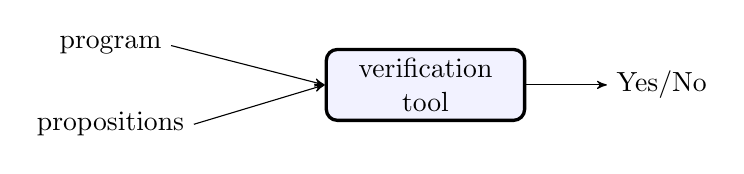
\begin{tikzpicture}
        \node[punkt] (tool) at (0,0) {verification\\tool};
        \node (program) at (-4,0.5) {program};
        \node (proposition) at (-4,-0.5) {propositions};
        \node (YN) at (3,0) {Yes/No};
        \path[->] (program.east) edge (tool.west)
                  (proposition.east) edge (tool.west)
                  (tool) edge (YN);
    \end{tikzpicture}
    \end{figure}
    and our target program has
    \begin{itemize}
        \item recursive data structure
        \item higher-order function
    \end{itemize}
\end{frame}

\newcommand{\map}{\m{map}}
\newcommand{\nil}{[\,]}

\begin{frame}
    \frametitle{Example Program}
    \begin{example}
            \setlength{\abovedisplayskip}{0pt}
            \setlength{\belowdisplayskip}{0pt}
        \begin{align*}
            \nil \catenate ys &= ys\\
            x\cons xs \catenate ys &= x \cons (xs \catenate ys)\\
            \map\,f\,\nil &= \nil\\
            \map\,f\,(x\cons xs) &= f\,x \cons (\map\,f\,xs)\\
        \end{align*}
        \vspace{-20pt}
    \begin{block}{Proposition}
        $\m{map}\,f\,(xs \catenate ys) = \m{map} \, f \, xs \catenate \m{map}\,f\,ys$
    \end{block}
        how to prove it? \quad \alert{induction}
    \end{example}
\end{frame}

\begin{frame}
    \begin{block}{Proposition}
        $\m{map}\,f\,(xs \catenate ys) = \m{map} \, f \, xs \catenate \m{map}\,f\,ys$
    \end{block}
    \begin{proof}
        by structural induction on $xs$
        \begin{itemize}
            \item if $xs = \nil$ $\m{map}\,f\,(\nil \catenate ys) = \m{map}\, f \,ys
                = \nil \catenate \m{map}\,f\,ys = \m{map}\,f\,\nil \catenate \m{map}\,f\,ys$
            \item if $xs = x \cons xs'$
            \setlength{\abovedisplayskip}{1pt}
            \setlength{\belowdisplayskip}{-1pt}
                \begin{align*}
                    \m{map}\,f(x\cons xs' \catenate ys) &= \m{map}\,f\,(x \cons (xs' \catenate ys))\\
                    &= f\,x \cons (\m{map}\,f\,(xs' \catenate ys))\\
                    &= f\,x \cons (\m{map}\,f\,xs' \catenate \m{map}\,f\,ys) \;\;\text{by I.H.}\\
                    &= f\,x \cons (\m{map}\,f\,xs') \catenate \m{map}\,f\,ys\\
                    &= \m{map}\,f\,xs \catenate \m{map}\,f\,ys
                \end{align*}
        \end{itemize}
        \vspace{-6pt}
    \end{proof}
\end{frame}

\begin{frame}
    \frametitle{What is Needed for Tool}
    propositions what we want to prove require \alert{induction}\\
    because date structures are \alert{recursive} (e.g. list, tree)\\
    so we need:
    \begin{figure}
        \centering
    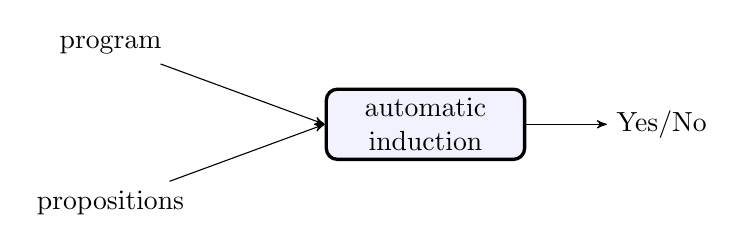
\begin{tikzpicture}
        \node[punkt] (tool) at (0,0) {automatic \\ induction};
        \node (program) at (-4,1) {program};
        \node (proposition) at (-4,-1) {propositions};
        \node (YN) at (3,0) {Yes/No};
        \path[->] (program) edge (tool.west)
                  (proposition) edge (tool.west)
                  (tool) edge (YN);
    \end{tikzpicture}
    \end{figure}
    \begin{itemize}
        \item how to do induction automatically? \quad \alert{rewriting induction}\\
        \item how to represent functions like $\m{map}$? \quad \alert{applicative term}
    \end{itemize}
\end{frame}

\begin{frame}
    \frametitle{Rewriting Induction}
    \begin{figure}
    \centering
    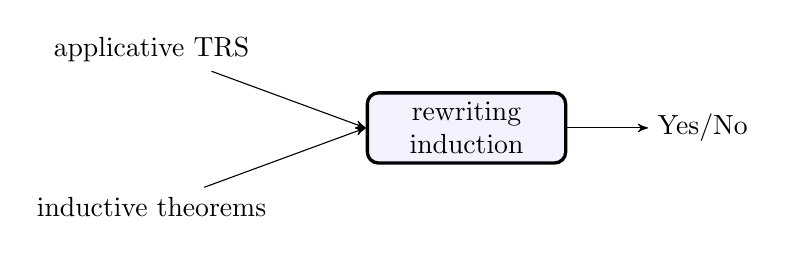
\begin{tikzpicture}
        \node[punkt] (tool) at (0,0) {rewriting \\ induction};
        \node (program) at (-4,1) {applicative TRS};
        \node (proposition) at (-4,-1) {inductive theorems};
        \node (YN) at (3,0) {Yes/No};
        \path[->] (program) edge (tool.west)
                  (proposition) edge (tool.west)
                  (tool) edge (YN);
    \end{tikzpicture}
    \end{figure}
    rewriting induction requires reduction order on applicative term
    \begin{itemize}
        \item lambda-free Knuth-Bendix order(2017) \quad based on KBO
        \item embedding path order (2021)
        \item applicative interpretation order (2023) \quad based on polynomial interpretation
    \end{itemize}
\end{frame}

\begin{frame}
    \frametitle{Limitation of Interpretation Method}
    \begin{example}
    polynomial order cannot orient
        \vspace{-1pt}
        \begin{align*}
            \m{ack}(\m{0}, y) &\to \m{s}(y)\\
            \m{ack}(\m{s}(x),\m{0}) &\to \m{ack}(x,\m{s}(\m{0}))\\
            \m{ack}(\m{s}(x),\m{s}(y)) &\to \m{ack}(x,\m{ack}(\m{s}(x),y))
        \end{align*}
    but Lexicographic path order can orient it
    \end{example}
\end{frame}

\begin{frame}
    \frametitle{Object of Research}
    \begin{itemize}
        \item develop new reduction order based on LPO
        \item develop rewriting induction on applicative term
    \end{itemize}
\end{frame}

\end{document}

